\documentclass{article}

\usepackage[most]{tcolorbox}
\usepackage{physics}
\usepackage{graphicx}
\usepackage{float}
\usepackage{amsmath}
\usepackage{amssymb}


\usepackage[utf8]{inputenc}
\usepackage[a4paper, margin=1in]{geometry} % Controla los márgenes
\usepackage{titling}

\title{Clase 13}
\author{Manuel Garcia.}
\date{\today}

\renewcommand{\maketitlehooka}{%
  \centering
  \vspace*{0.05cm} % Espacio vertical antes del título
}

\renewcommand{\maketitlehookd}{%
  \vspace*{2cm} % Espacio vertical después de la fecha
}

\newcommand{\caja}[3]{%
  \begin{tcolorbox}[colback=#1!5!white,colframe=#1!25!black,title=#2]
    #3
  \end{tcolorbox}%
}

\begin{document}
\maketitle

\section{Funcion Analitica }
En el calculo real las funciones usualmente se definen en intervalos, en el caso de la variable compleja los intervalos son reemplazados por subconjuntos del espacio complej. Dichos subconjuntos tienen las siguientes propiedades: 
\begin{itemize}
  \item \textbf{Definicion Vecindades: } sea $ r > 0  $ y $ z_0 $ un numero complejo en el plano. La vecindad $ r  $ de $ z_0  $ es el conjunto de todos los numeros complejos que satisfacen $ \left|z-z_0\right|<r  $. Convencionalmente este conjunto lo denotamos como: $ B_r(z_0 ) $. Demonos cuenta que los puntos que forman el perimetro no están incluidos. 

    Vamos a definir, adicionalmente, una \textbf{Vecindad Puntuada} $ B_r'(z_0 ) $ y cumple  $ B_r' (z_0) = \{z : 0<\left|z-z_0 \right|<r \} $, es decir $ z_0 $ no pertenece al conjunto.
  \item \textbf{Definicion: } Sea $ S  $ un subconjunto de $ \mathbb{C} $. Un punto $ z_0  $ en $ S  $ es llamado un \textbf{punto interior} de $ S  $ si podemos encontrar una vecindad de $ z_0  $ que esté totalmente contenida en $ S  $. Un punto $ z  $ se llamará \textbf{punto de frontera} de $ S  $ si toda vecindad de $ z  $ contiene al menos un punto interior y un punto en el exterior de $ S  $.
  \begin{figure}[H]
    \begin{center}
      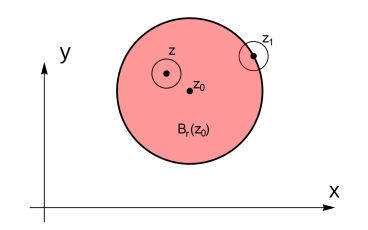
\includegraphics[width=0.5\textwidth]{frontera.png}
    \end{center}
  \end{figure}

  \item \textbf{Definicion conjuntos abiertos: } Un conjunto $S  $ d enumeros complejos se llamará \textbf{abierto }, si todos los puntos que los conforman son interiores. 
  \begin{itemize}
    \item Vecindad, $ B_r(z_0) $ es un conjunto abierto. 
    \item El ocnjunto $S = \{z: \left|z-z_0 \right|>r\}$, es una vecindad al infinito y es un conjunto abierto. 
    \item El conjunto cerrado más "pequeño" que contiene a un conjunto $ A  $ se llamará la cerradura de $ A  $. 

    Por ejemplo: sea un disco abierto $ B_r (z_0)  $, entonces su cerradura es : 
    \begin{gather*}
      \bar{B_r(z_0)} = \{z: \left|z-z_0 \right|\leq r \}
    \end{gather*}
  \end{itemize}
  \item \textbf{Definicion: } Un \textbf{punto de acumulacion } de un conjunto $ A  $, $ z_0  $, será aquel que cumpla $ B_r'(z_0) \cap A \neq \emptyset  $, para cualquier $ r>0  $.
    \begin{figure}[H]
      \begin{center}
        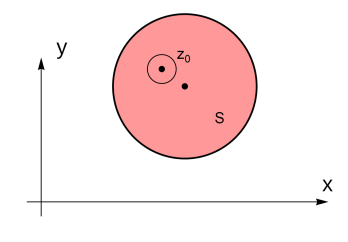
\includegraphics[width=0.5\textwidth]{punto_acumulacion.png}
      \end{center}
    \end{figure}
\end{itemize}

\caja{black}{}{
  \begin{gather*}
    A\cup B = \{z: z \in A \lor z \in B \}\\
    A\cap B = \{z: z\in A \land z\in B \}\\
    A-B = \{ z: z\in A \land z \notin B \}
  \end{gather*}
}

\subsection{Conjunto conexo }
Un resultado de cálculo real es que la derivada de una función es un intervalo abierto que sea cero, implica que la función es constante. Tengamos presente que este resultado no es valido si el conjunto no es conexo. 

\textbf{Ej: }
\begin{gather*}
  g(t) = 
     \begin{cases}
       1 &\text{si } 0 <t<5\\
       -1 &\text{si } 7 <t<10\\
     \end{cases} 
\end{gather*}
$ g'(t) $ en el intervalo $ (0,5)\cup (7,10) $ es cero, sin embarlo la funcion no es constante.

\begin{itemize}
  \item \textbf{Definicion: } Una \textbf{Linea poligonal } es una union finita de segmento de linea recta, cuyos extremos finales los denotamos como $ L_J, \quad J = 1,2,3,...  $
    \begin{figure}[H]
      \begin{center}
        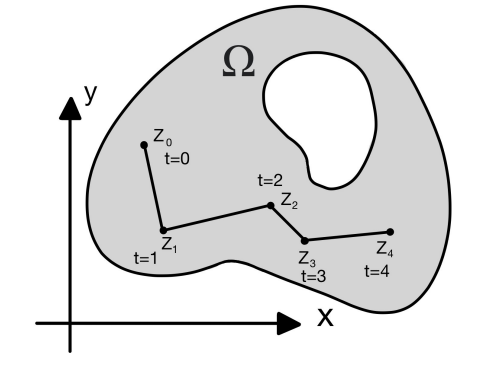
\includegraphics[width=0.3\textwidth]{linea_poligonal.png}
      \end{center}
    \end{figure}
  Esto nos permite definir un subconjunto poligonalmente conexo.
\end{itemize}

\subsection{Limites y continuidad}
\begin{itemize}
  \item \textbf{Funciones univaluadas: }Definamos en este contexto el límite de una función $ f(z)  $ cuando z se acerca a $ z_0  $ como $ L  $, si: 
    \begin{gather*}
      z \in S \quad \land \quad 0<\left|z-z_0 \right|<\delta \implies \left|f(z) - L \right| < \epsilon 
    \end{gather*}
    \begin{figure}[H]
      \begin{center}
        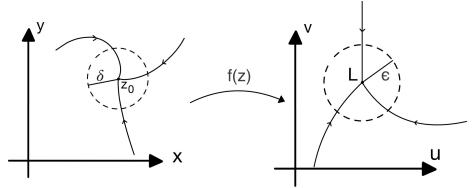
\includegraphics[width=0.6\textwidth]{lim_univaluada.png}
      \end{center}
    \end{figure}
    \textbf{Ejercicio: }Demuestre a traves de $ \epsilon $ y $ \delta $ que: $ \underset{z \rightarrow 2+3i }{lim } 5z + 3 = 13 + 15i $.
    \textbf{Sol: } tenemos que $ 0<\left|z-(2+3i)\right|<\delta $, $ \left|(5z + 3 ) - (13 + 15i)\right|<\epsilon \rightarrow \left|5z - 10 + 15i \right|<\epsilon \rightarrow \left|z - (2 + 3i )\right|< \epsilon/5$. Para dado $ \epsilon $ tenemos que $ \delta = \epsilon/5 $
\end{itemize}
\caja{black}{Ejercicio }{
  Demostrar con $ \epsilon $ y $ \delta $ que: 
  \begin{gather*}
    \underset{z \rightarrow i }{lim }\frac{3z^4 - 2 z^3 + 8z^2 - 2z + 5 }{z-i } = 4 + 4i 
  \end{gather*}
}

\end{document}
